\documentclass[12pt]{article}
\setlength\parindent{0pt}
\usepackage{fullpage}
\usepackage[paperwidth=14in, paperheight=9in, textwidth=12in, textheight=8in]{geometry}
\usepackage{amsmath}
\usepackage{graphicx}
\setlength{\parskip}{4mm}
\def\LL{\left\langle}   % left angle bracket
\def\RR{\right\rangle}  % right angle bracket
\def\LP{\left(}         % left parenthesis
\def\RP{\right)}        % right parenthesis
\def\LB{\left\{}        % left curly bracket
\def\RB{\right\}}       % right curly bracket
\def\PAR#1#2{ {{\partial #1}\over{\partial #2}} }
\def\PARTWO#1#2{ {{\partial^2 #1}\over{\partial #2}^2} }
\def\PARTWOMIX#1#2#3{ {{\partial^2 #1}\over{\partial #2 \partial #3}} }
\newcommand{\BE}{\begin{displaymath}}
\newcommand{\EE}{\end{displaymath}}
\newcommand{\BNE}{\begin{equation}}
\newcommand{\ENE}{\end{equation}}
\newcommand{\BEA}{\begin{eqnarray}}
\newcommand{\EEA}{\nonumber\end{eqnarray}}
\newcommand{\EL}{\nonumber\\}
\newcommand{\la}[1]{\label{#1}}
\newcommand{\ie}{{\em i.e.\ }}
\newcommand{\eg}{{\em e.\,g.\ }}
\newcommand{\cf}{cf.\ }
\newcommand{\etc}{etc.\ }
\newcommand{\Tr}{{\rm tr}}
\newcommand{\etal}{{\it et al.}}
\newcommand{\OL}[1]{\overline{#1}\ } % overline
\newcommand{\OLL}[1]{\overline{\overline{#1}}\ } % double overline
\newcommand{\OON}{\frac{1}{N}} % "one over N"
\newcommand{\OOX}[1]{\frac{1}{#1}} % "one over X"



\begin{document}
\Large
\centerline{\sc{Recitation Questions}}
\normalsize
\centerline{\sc{April 24}}

\begin{enumerate}

\item A flywheel (a large, spinning disc) of mass $m$ and radius $r$ is rotating
at angular velocity $\omega$. The machine operator wishes to bring it to rest using a brake. When the brake 
is engaged, two brake pads on either side of the disc are pressed against it from either side, two-thirds
of the way from the center to the outer edge; each brake pad
exerts a normal force $F_N$. 

If the coefficient of friction between the brake pads and the disc is $\mu_k$, how long does it take the
brake to bring the flywheel to a stop?


\newpage

\begin{center} \it This question appeared on last year's final exam. There is another copy of the diagram on a blank page after this one for you to write on.\end{center}

\item A student from last semester, Nataly, has an enormous cat named Reesie. He is always getting himself into trouble. You may model Reesie as a thin, straight, uniform rod that is 90 cm long and has a mass of 10 kg.

\begin{minipage}{0.6\textwidth}
	It is well-known that cats are unable to resist knocking things over.\footnotemark~Nataly leaves a pitcher of water resting on a stool 75 cm tall. Upset that he's only gotten
	one dinner so far tonight, Reesie
	stands on his back paws and leans on the base of the pitcher with his front paws, trying to knock it off the stool. Since Reesie is standing on carpet and has claws, he can grip the carpet with whatever force is required to keep his back paws in place; his rear paws act as a hinge. Since his front paws are very fuzzy and the side of the glass is smooth, there is no frictional force between the glass and the front paws; the force from the glass on the cat is purely horizontal.
	
	\bigskip
	
	The coefficient of static friction between the pitcher and the stool is $\mu_s = 0.5$.
	
	\bigskip
	\bigskip
	
	\begin{itemize}
		\item What is the most massive pitcher of water that Reesie could push off the stool?
		\item Determine the force that Reesie's rear claws exert on the carpet when he does this.
	\end{itemize}
\end{minipage}
\begin{minipage}{0.4\textwidth}
	\begin{center}
		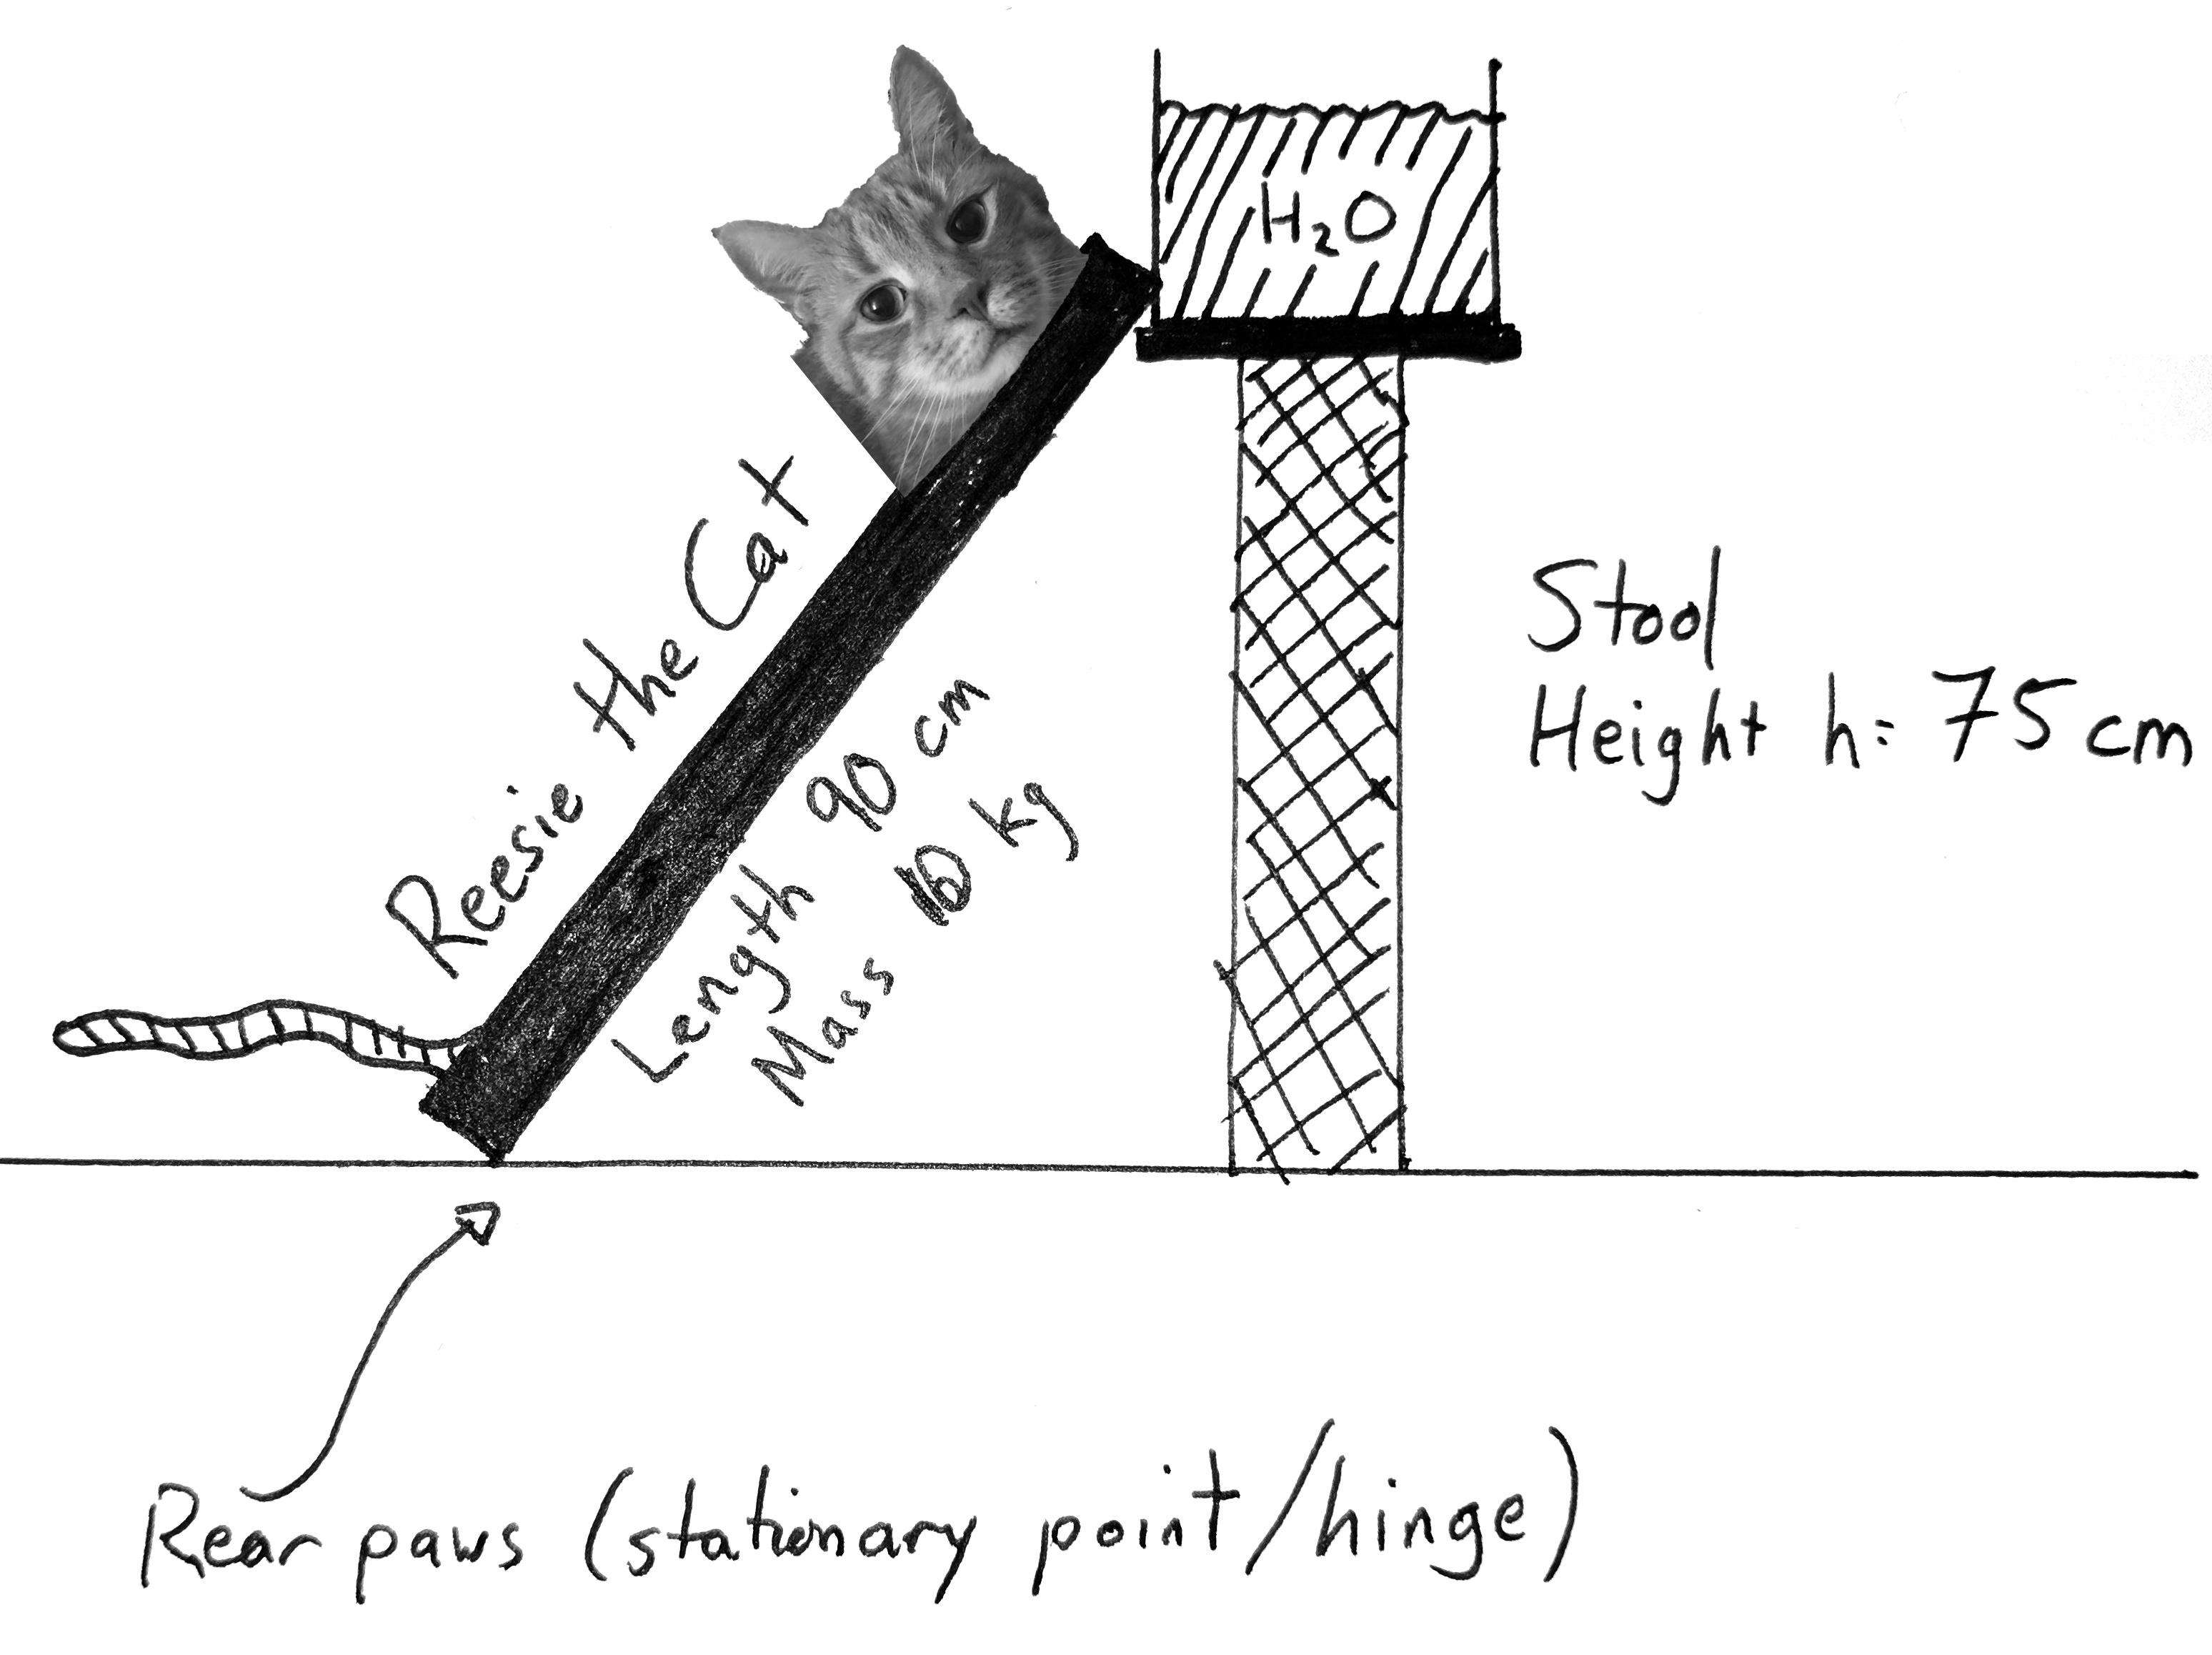
\includegraphics[width=0.95\textwidth]{reesie-diagram.jpg}
	\end{center}
\end{minipage}
\footnotetext{``We know the world isn't flat. If it were, cats would have pushed everything off it by now.'' Yet another example of flat-earthers ignoring refuting evidence...}
\vfill

\newpage

	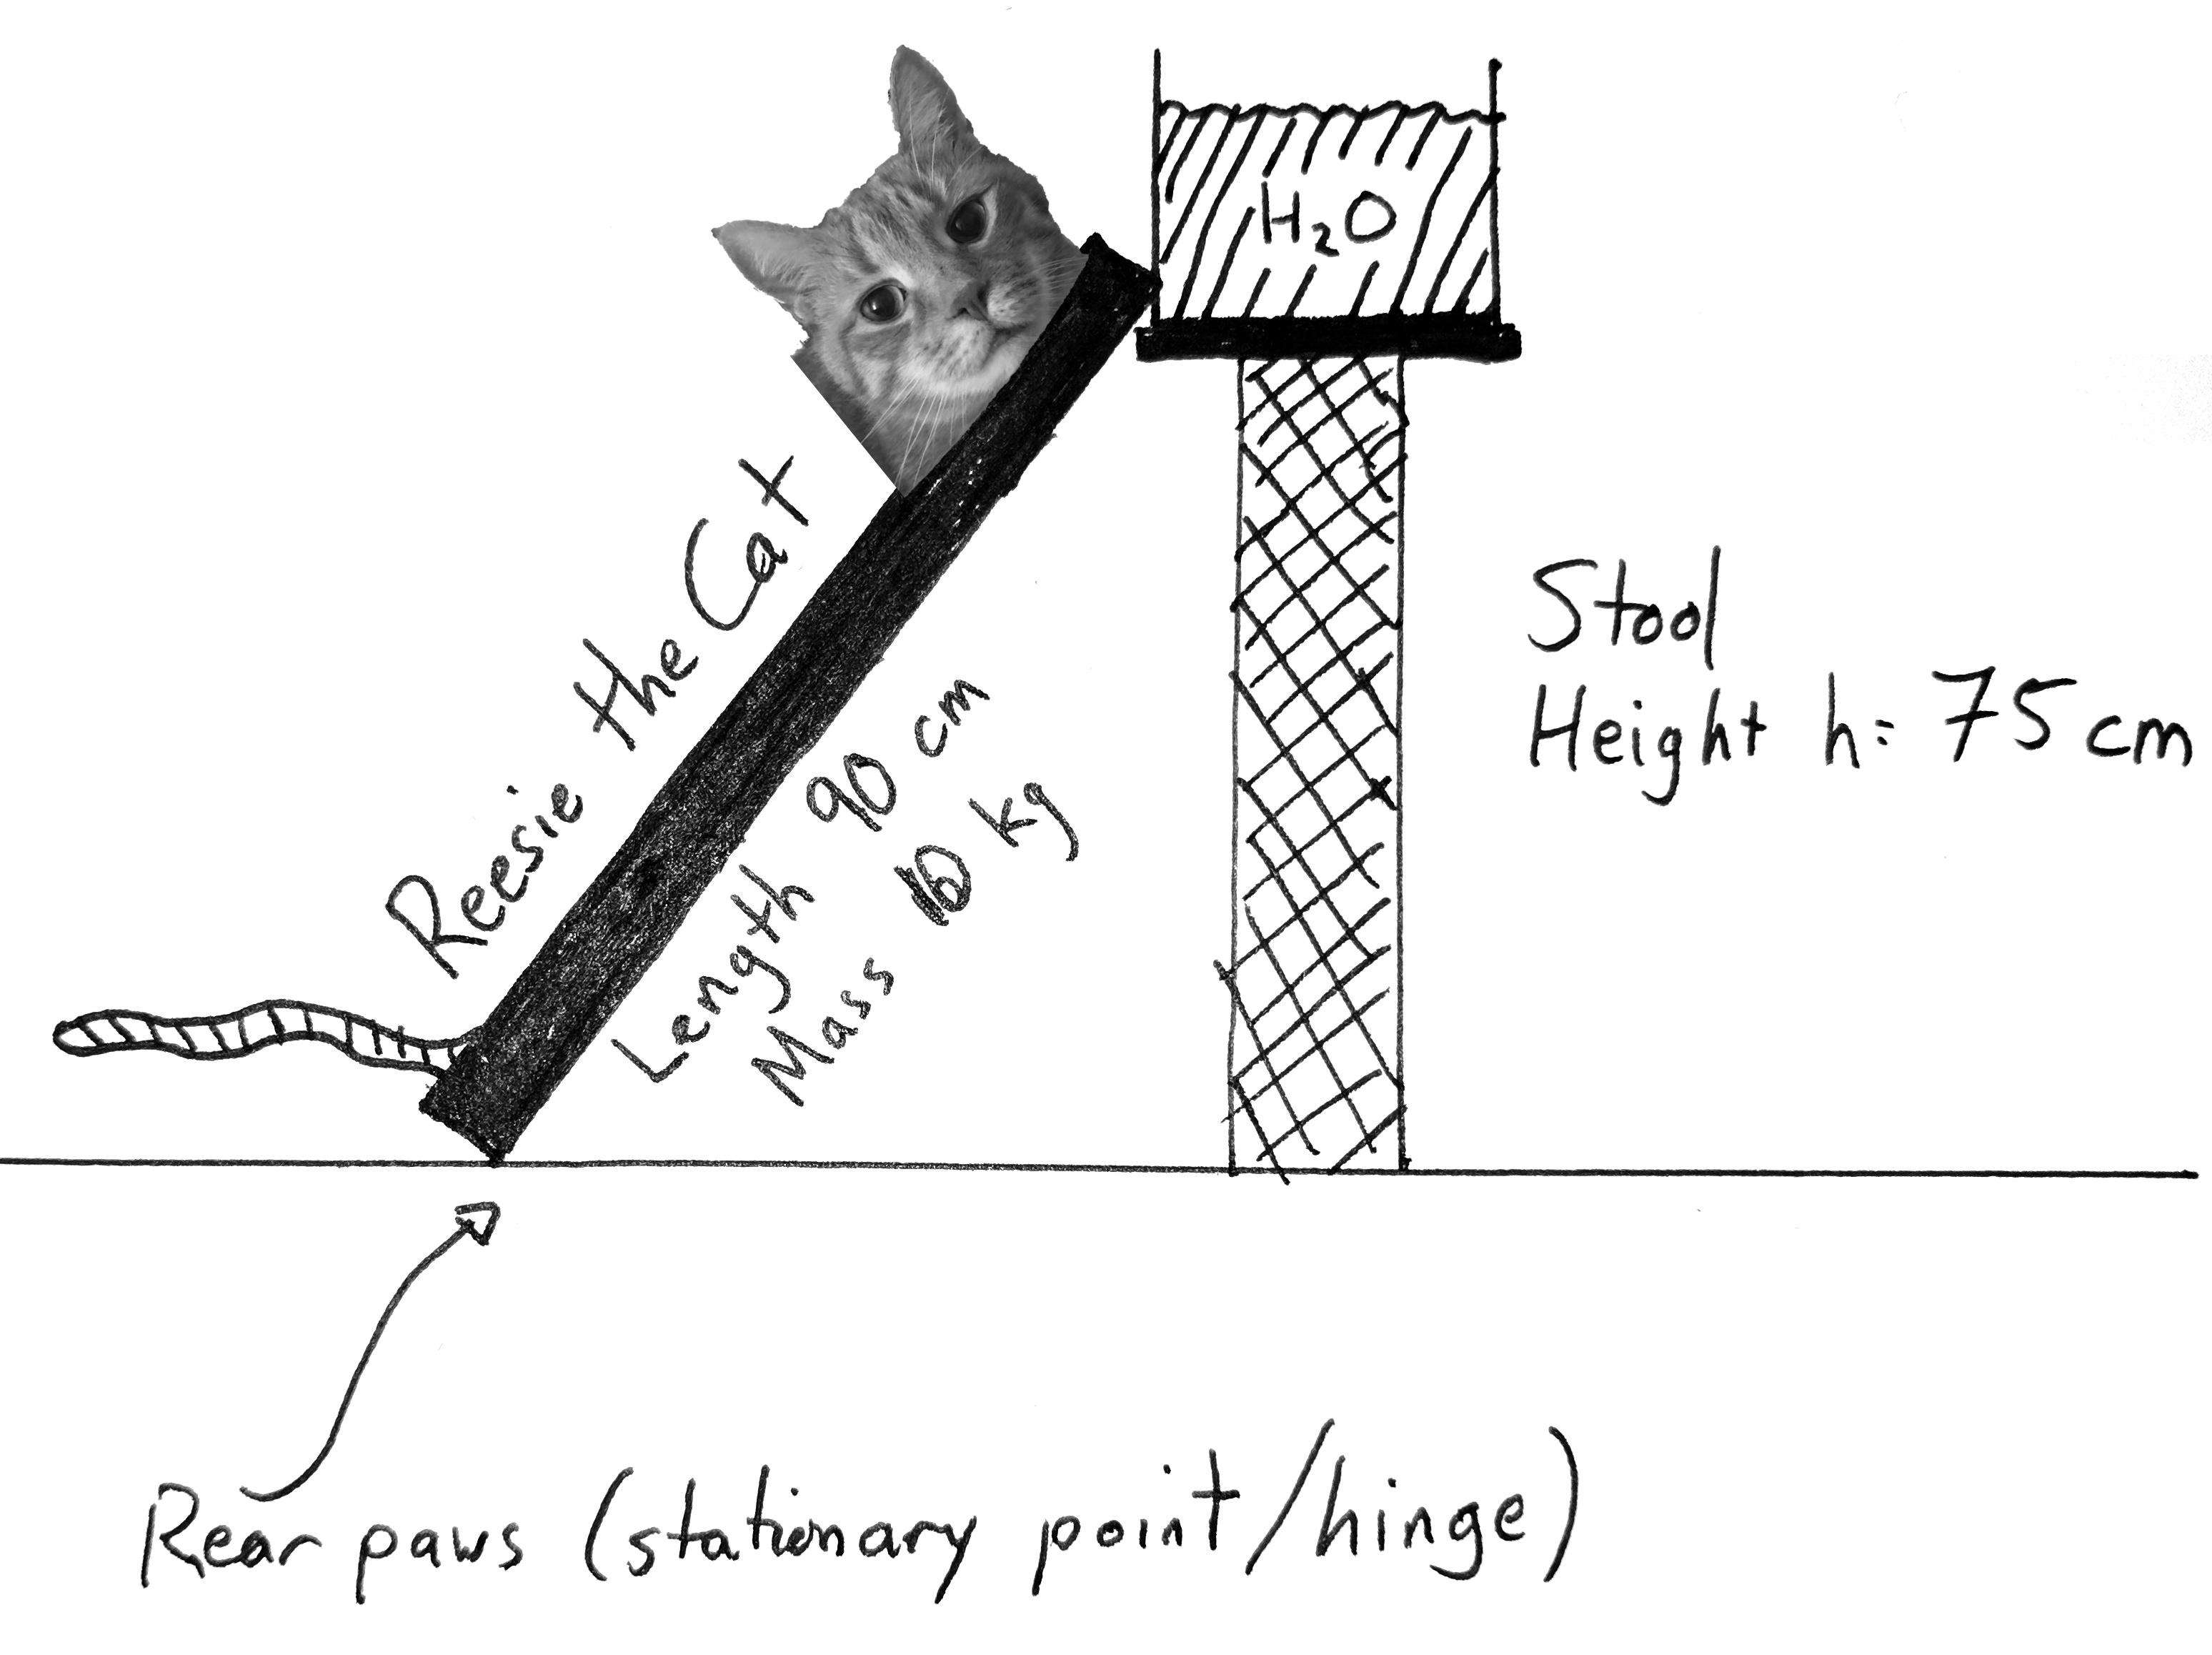
\includegraphics[width=0.4\textwidth]{reesie-diagram.jpg}
	
	\newpage
	
	
	
   \item{A Yo-Yo consists of a cylinder of mass $m$ and radius $r$. A slot is cut in the middle of the cylinder such that the inner radius is only $0.4r$, and a string is wound around the middle. 
     A person holds the string and allows the Yo-Yo to fall. As it falls, it has both a linear acceleration (moving downward) and an angular acceleration (spinning faster and faster). In this problem, you will find them.}
     \begin{enumerate}
     	
     	       \item{Draw a force diagram for the Yo-Yo, indicating the location where all forces act as well as their magnitude.}
     	
     	\vspace{4in}
     	
       \item{What is the relation between the linear velocity $v$ of the Yo-Yo (moving downward) and its angular velocity $\omega$?}

\vspace{1in}
       \item{What is the relation between the linear acceleration $a$ of the Yo-Yo (moving downward) and its angular acceleration $\alpha$? (Note: this is trivial once you've done the previous part...)}

\vspace{1in}


\newpage
       \item{Write down Newton's second law ($F=ma$) for the Yo-Yo, putting in expressions for the various forces.}

\vspace{2in}

       \item{Write down ``Newton's second law for rotation'' $\tau = I \alpha$, putting in expressions for the net torque and the moment of inertia.}

\vspace{2in}
       \item{What is the acceleration of the Yo-Yo and the tension in the string?}

\vspace{2.5in}
       \item{Will the Yo-Yo accelerate faster or slower if the inner radius is changed to $0.2r$?}


     \end{enumerate}

\newpage
\centerline{\sc{Reference Material - Rotational Motion}}


Moments of Inertia:
\begin{itemize}
  \item{Disk or cylinder, rotating about center: $I = \frac{1}{2}MR^2$}
  \item{Sphere, rotating about center: $I = \frac{2}{5}MR^2$}
  \item{Ring or hollow cylinder, rotating about center: $I = MR^2$}
\end{itemize}

\bigskip
\bigskip
\bigskip

Correspondence between linear dynamics and rotational dynamics: 
  \scriptsize

\begin{tabular}{| c | c | c | c |}
  \hline
  Position & $s$ & Angle & $\theta$  \\
  Velocity & $\vec v$ & Angular velocity & $\omega$  \\
  Acceleration & $\vec a$ & Angular acceleration & $\alpha$  \\
  \hline
                                   & $v(t) = v_0 + at$ & & $\omega(t) = \omega_0 + \alpha t$ \\
                                   & $x(t) = x_0 + v_0 t + \frac{1}{2} at^2$ & & $\theta(t) = \theta_0 + \omega_0 t + \frac{1}{2} \alpha t^2$ \\
                                   & $v_f^2 - v_0^2 = 2a \Delta x$ & & $\omega_f^2 - \omega_0^2 = 2 \alpha \Delta \theta$ \\
  \hline
  Mass & $m$ & Moment of inertia & $I$ \\
  \hline
  Force & $F$ & Torque & $\tau = F_\perp r = F r_\perp$ \\
  \hline
  Newton's second law & $\vec F = m \vec a$ & ``Newton's second law for rotation'' & $\tau = I \alpha$ \\
  \hline
  Kinetic energy & $\frac{1}{2} mv^2$ & Kinetic energy & $\frac{1}{2}I\omega^2$ \\
  \hline
  Momentum & $\vec p = m \vec v$ & Angular momentum & $L = I \omega$ \\
  \hline
\end{tabular}

\bigskip
\bigskip
\bigskip

Arc length $s=\theta r$ \\
Tangential velocity $v=\omega r$ \\
Tangential acceleration $a=\alpha r$




 \end{enumerate}
 \end{document}
